\section{Estructura Jerárquica} % (fold)
\label{sec:estructura_jerarquica_impl}
La representación de la escena en vóxeles puede ser filtrada hacia niveles menos detallados utilizando distintos niveles de mip map. Esto describe una estructura piramidal. Esta estructura es utilizada para acelerar el trazado de conos contra vóxeles, donde según la apertura del cono se interpola entre distintos niveles de detalle como se observa en la Figura \ref{fig:vct_explain}.

En nuestra implementación se utilizan seis nuevos volúmenes por cada eje direccional positivo y negativo para vóxeles anisótropos. Cada uno de estos volúmenes tiene una resolución de $V_{res}/{2}$. Los niveles de mipmapping no se encuentran en la textura base de radiancia sino en estos volúmenes, por tanto estos volúmenes son los que residen los distintos niveles de detalle de la escena voxelizada. Llamaremos a estos volúmenes como \emph{volúmenes direccionales}. En la Figura \ref{fig:base_texture_imp} se ilustra esta separación.

Como utilizamos texturas tridimensionales en vez de un octree el proceso de filtrado es mucho más simple ya que la interpolación cuadrilineal esta soportada nativamente. Un problema surge para la interpolación entre la textura base y los niveles de mipmapping en los volúmenes direccionales. Ya que estas son texturas separadas no hay interpolación lineal entre la textura base y los volúmenes direccionales. Esto es simple de solventar utilizando la función \emph{mix()} de GLSL cuando el nivel de detalle se encuentre entre cero y uno, cero siendo el máximo detalle (textura base) y uno el nivel cero del mipmap en los volúmenes direccionales. La Figura \ref{fig:hierarchy_impl} describe esta estructra.

\begin{figure}[H]
    \centering
    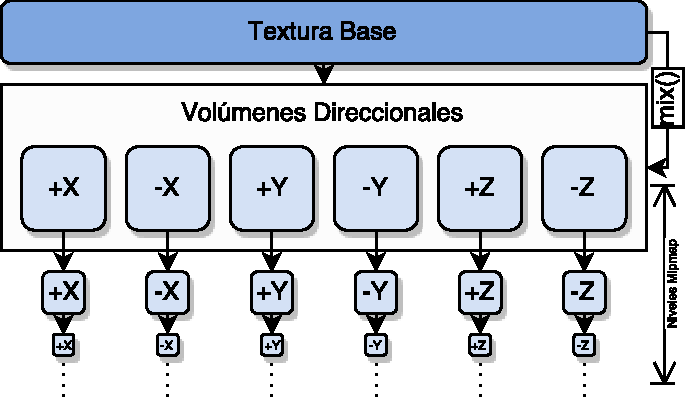
\includegraphics[width=.8\linewidth]{media/hierarchy.pdf}
    \caption{Descripción gráfica de la estructura jerárquica de vóxeles utilizada para el trazado de conos.}
    \label{fig:hierarchy_impl}
\end{figure}

\begin{figure}[H]
    \centering
    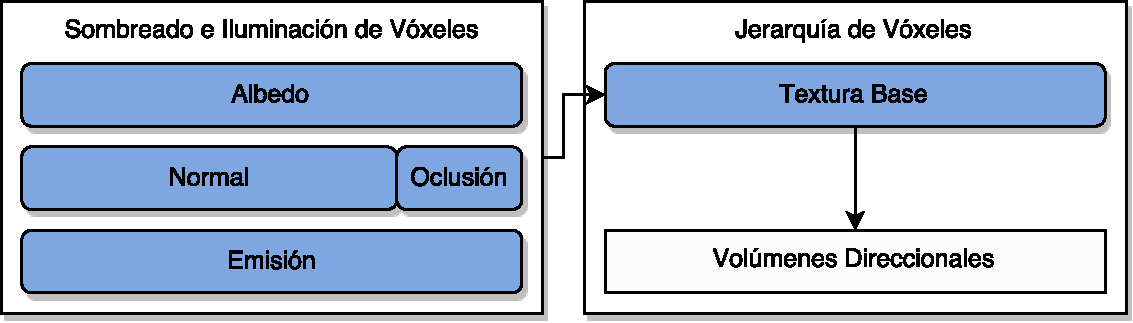
\includegraphics[width=.8\linewidth]{media/representation.pdf}
    \caption{Representación de la escena en vóxeles. La textura base es producto de cálculos de iluminación sobre las texturas utilizadas durante el sombreado de vóxeles.}
    \label{fig:base_texture_imp}
\end{figure}
\subsection{Vóxeles Anisótropicos} % (fold)
\label{sub:voxeles_anisotropos}
El proceso para generar vóxeles anisótropicos es explicado de forma general en la sección \ref{subsub:aniso_voxels_orig}. Una representación con vóxeles anisótropicos provee mayor calidad visual y precisión durante el trazado de conos. Cada cono trazado tiene una dirección, la idea es utilizar esta dirección para saber cuáles volúmenes direccionales van a utilizarse para interpolar. Para una dirección arbitraria esto representa tres volúmenes que serían las caras frontales según esta dirección del vóxel simplificado. La dirección del cono tiene un peso en cada eje direccional, por tanto los valores de cada uno de estos volúmenes direccionales deben ser ponderados al momento de muestrearse. Una representación isótropa no tiene concepto de direccionalidad del cono, por tanto para algunos casos esto puede generar una serie de problemas visuales ya mencionados. Las desventajas de esta implementación es que el trazado es más lento ya que se deben realizar tres muestras por cada paso del cono y mayor consumo de memoria.

Una forma simplificada de observar este proceso es con texturas bidimensionales. Suponiendo que tenemos una cuadrícula de $5^2$ que queremos reducir a un nivel de detalle más bajo de $3^2$ como se observa en la Figura \ref{fig:filter_objs}.

\begin{figure}[H]
    \centering
    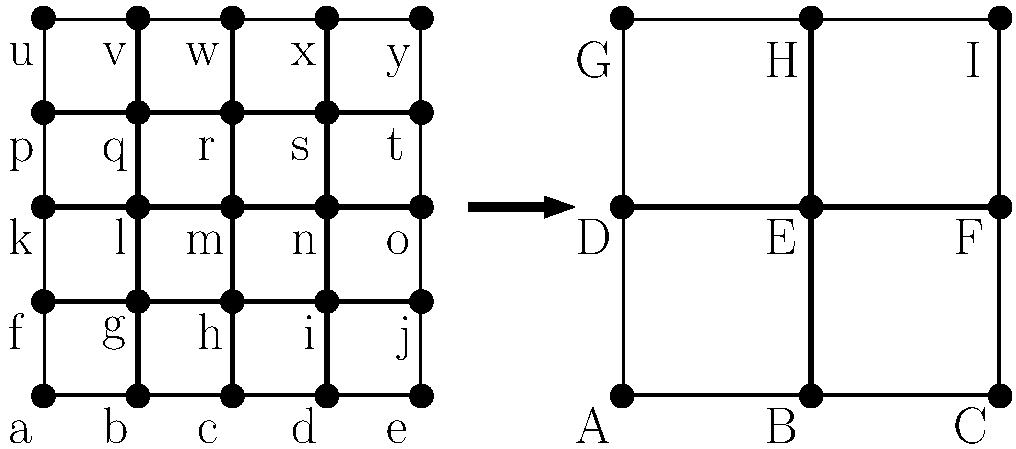
\includegraphics[width=.5\linewidth]{media/filtering_1.pdf}
    \caption{Cuadrícula de vóxeles de $5^2$ a menor detalle $3^2$.}
   	\label{fig:filter_objs}
\end{figure}

Para filtrar el valor del vóxel $E$ en la dirección $X$ positiva es necesario considerar los nueve vóxeles cercanos en el nivel anterior de detalle. Estos vóxeles son divididos en grupos de cuatro como se observa en la Figura \ref{fig:filter_groups}.

\begin{figure}[H]
    \centering
    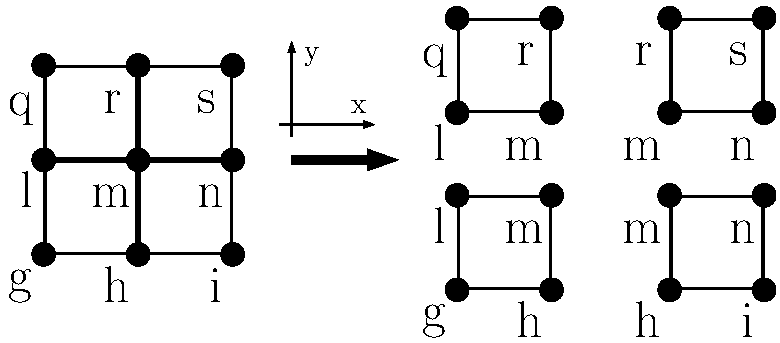
\includegraphics[width=.5\linewidth]{media/filtering_2.pdf}
    \caption{Separación de vóxeles cercanos a $E$ en grupos a filtrar.}
    \label{fig:filter_groups}
\end{figure}

Por cada grupo se filtra en la dirección $X$ positiva. Por ejemplo en el primer grupo, en la parte superior izquierda. Primero se realiza mezclado alfa o \emph{alpha blending} en la dirección $X$ positiva y luego se calcula un promedio para obtener el valor de este grupo. La siguiente ecuación describe este proceso:
\smallskip
\begin{equation}
\begin{split}
	\begin{pmatrix}R\\G\\B\\A\end{pmatrix}_{q \to r} &= 
	\begin{pmatrix}R\\G\\B\\1\end{pmatrix}_{r}A_{r} +
	\begin{pmatrix}R\\G\\B\\A\end{pmatrix}_{q}(1-A_{r})\\
	\begin{pmatrix}R\\G\\B\\A\end{pmatrix}_{l \to m} &= 
	\begin{pmatrix}R\\G\\B\\1\end{pmatrix}_{m}A_{m} +
	\begin{pmatrix}R\\G\\B\\A\end{pmatrix}_{l}(1-A_{m})\\
	\begin{pmatrix}R\\G\\B\\A\end{pmatrix}_{q \to r, l \to m} &= 
	\begin{bmatrix}
	\begin{pmatrix}R\\G\\B\\A\end{pmatrix}_{q \to r} +
	\begin{pmatrix}R\\G\\B\\A\end{pmatrix}_{l \to m}
	\end{bmatrix}\cdot 0.5
\end{split}
\end{equation}

Una vez se obtiene cada valor de los cuatro grupos se puede ahora calcular el valor del vóxel filtrado repitiendo este proceso con los cuatro valores resultantes. En nuestra implementación esto se realiza con un compute shader. El Código \ref{AnisoFiltering} expone este proceso sobre texturas tridimensionales.
\\
\begin{lstlisting}[caption={Filtrado sobre los volúmenes direccionales para obtener vóxeles anisótropos}, label=AnisoFiltering]
(*@\centerline{\raisebox{-1pt}[0pt][0pt]{$\vdots$}}@*)
// posiciones de vóxeles cercanos
const ivec3 anisoOffsets[] = ivec3[8]
(
	ivec3(1, 1, 1),
	ivec3(1, 1, 0),
	ivec3(1, 0, 1),
	ivec3(1, 0, 0),
	ivec3(0, 1, 1),
	ivec3(0, 1, 0),
	ivec3(0, 0, 1),
	ivec3(0, 0, 0)
);
// obtiene vóxeles cercanos
void FetchTexels(ivec3 pos, int dir, inout vec4 val[8]) 
{
	for(int i = 0; i < 8; i++)
	{
		val[i] = texelFetch(voxelMipmapSrc[dir], pos + anisoOffsets[i], mipLevel);
	}
}
void main()
{
	if(gl_GlobalInvocationID.x >= mipDimension.x ||
		gl_GlobalInvocationID.y >= mipDimension.y ||
		gl_GlobalInvocationID.z >= mipDimension.z) return;

	// posición de escritura
	ivec3 writePos = ivec3(gl_GlobalInvocationID);
	// posición de lectura, mip de mayor detalle
	ivec3 sourcePos = writePos * 2;
	// Arreglo de valores cercanos a filtrar
	vec4 values[8];
	// obtiene valores del volumen -X
	FetchTexels(sourcePos, 0, values);
	// filtrado en dirección -X
	imageStore(voxelMipmapDst[0], writePos, 
	(
		values[0] + values[4] * (1 - values[0].a) + // Mezclado Alfa
		values[1] + values[5] * (1 - values[1].a) +
		values[2] + values[6] * (1 - values[2].a) +
		values[3] + values[7] * (1 - values[3].a)) * 0.25f // Promedio
	);
	// obtiene valores del volumen +X
	FetchTexels(sourcePos, 1, values);
	// filtrado en dirección +X
    imageStore(voxelMipmapDst[1], writePos, 
	(
		values[4] + values[0] * (1 - values[4].a) + 
    	values[5] + values[1] * (1 - values[5].a) +
    	values[6] + values[2] * (1 - values[6].a) +
    	values[7] + values[3] * (1 - values[7].a)) * 0.25f
    );
	// obtiene valores del volumen -Y
	FetchTexels(sourcePos, 2, values);
	// filtrado en dirección -Y
    imageStore(voxelMipmapDst[2], writePos, 
	(
		values[0] + values[2] * (1 - values[0].a) +
    	values[1] + values[3] * (1 - values[1].a) +
    	values[5] + values[7] * (1 - values[5].a) +
    	values[4] + values[6] * (1 - values[4].a)) * 0.25f
    );
	// obtiene valores del volumen +Y
	FetchTexels(sourcePos, 3, values);
	// filtrado en dirección +Y
    imageStore(voxelMipmapDst[3], writePos, 
	(
		values[2] + values[0] * (1 - values[2].a) +
    	values[3] + values[1] * (1 - values[3].a) +
    	values[7] + values[5] * (1 - values[7].a) +
    	values[6] + values[4] * (1 - values[6].a)) * 0.25f
    );
	// obtiene valores del volumen -Z
	FetchTexels(sourcePos, 4, values);
	// filtrado en dirección -Z
    imageStore(voxelMipmapDst[4], writePos, 
	(
		values[0] + values[1] * (1 - values[0].a) +
    	values[2] + values[3] * (1 - values[2].a) +
    	values[4] + values[5] * (1 - values[4].a) +
    	values[6] + values[7] * (1 - values[6].a)) * 0.25f
    );
	// obtiene valores del volumen +Z
	FetchTexels(sourcePos, 5, values);
	// filtrado en dirección +Z
    imageStore(voxelMipmapDst[5], writePos, 
	(
		values[1] + values[0] * (1 - values[1].a) +
    	values[3] + values[2] * (1 - values[3].a) +
    	values[5] + values[4] * (1 - values[5].a) +
    	values[7] + values[6] * (1 - values[7].a)) * 0.25f
    );
}
\end{lstlisting}

Este proceso se repite por cada nivel mip de las texturas direccionales. Estas son enlazas según el nivel mip que va a ser filtrado con la instrucción \emph{glBindImageTexture}. La variable \emph{mipLevel} le indica a la instrucción \emph{texelFetch} cual es el nivel anterior de detalle como fuente de filtrado. Cuando se filtra desde la textura base al nivel 0 de los volúmenes direccionales el proceso es similar. La diferencia reside en dos detalles: primero solo se hace una llamada a \emph{FetchTexels} porque solo hay una textura fuente y segundo que el \emph{mipLevel} es cero ya que la textura base no tiene mip mapping y esta representa el máximo nivel de detalle de la estructura jerárquica.


% subsection voxeles_anisotropos (end)
% section estructura_jerarquica (end)
